\subsection{Implementation of Dijkstra's Algorithm} \label{implementation}
Our implementation of Dijkstra's algorithm can be viewed as generating a matrix, where one column of the matrix represents one state during the execution of the algorithm. Each column stores the original input graph, source node, a vector of currently unexplored node, and a vector of current distance value for all nodes in the graph, and a new column is calculated based on the value stored in the last column generated. The \inl{Column} data type in the data structure section (section \ref{column}) is defined for this column representation. However, since the calculation of a new column does not requires all previous columns calculated, and in order to simplify the data structures, the implementation does not maintain the whole matrix, rather, only one variable of the \inl{Column} data type is maintained to store the last column calculated. 
\\

Even though the whole matrix is not presented, we can still visualize this implementation as generating a matrix representation of Dijkstra's algorithm, where the columns shows how distance value of all nodes in the graph is gradually updated, hence in the following sections we still refers= to this matrix representation of Dijkstra's algorithm, based on the above clarification that the actual matrix is not presented in the implementation. Eliminating the matrix structure not only reduces some redundancy in our implementation, but also allows us to verify Dijkstra's algorithm by proving properties over each \inl{Column} calculated, which provides a clear structure for our verification program.

\begin{figure}[H]
	\centering
	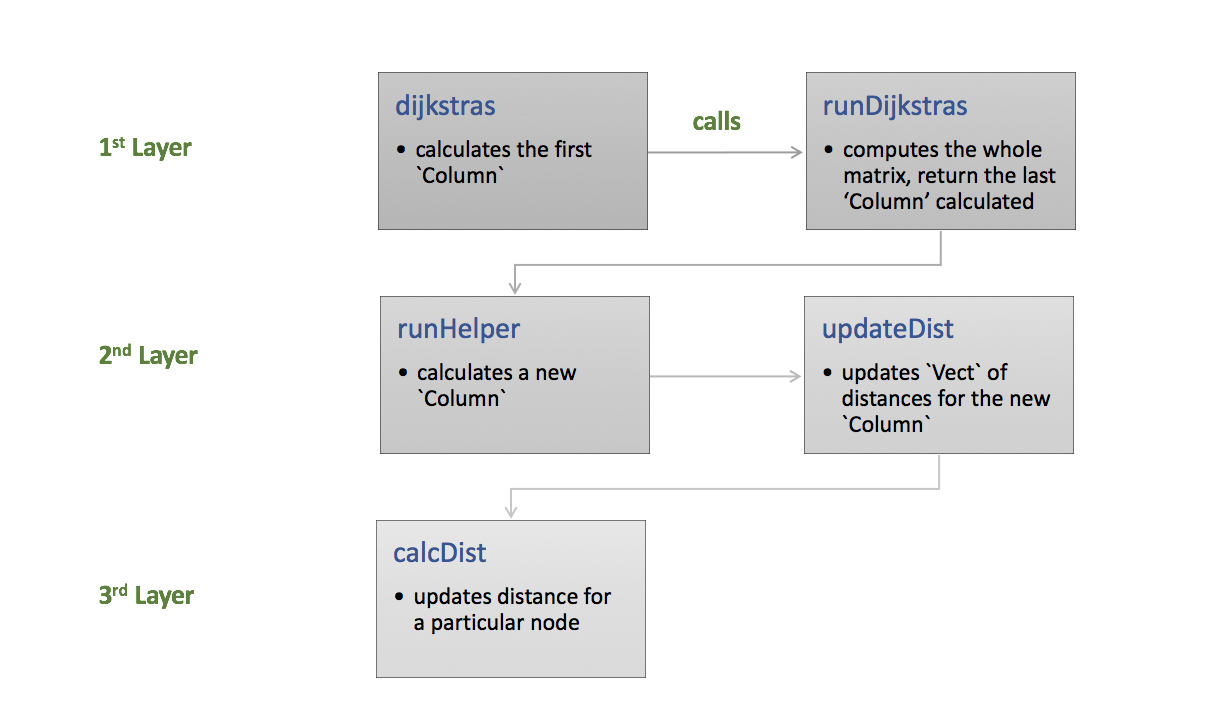
\includegraphics[scale = 0.6]{./figure/dijkstras_funcs.png}
	\caption{Structure of Dijkstra's Implementation}
	\label{figure3}
\end{figure}

As illustrated by Figure \ref{figure3} above, the implementation can be divided into three layers, where each layer breaks down the calculation to deal with a smaller structure. Specifically, the first layer calculates the whole matrix representation by calling function from the second layer. The second layer is responsible for generating a new \inl{Column} data based on the last \inl{Column} calculated, where the updated distance value for each node in the graph is calculated by the third layer. The remaining of this section provides more details on our three layers of calculation. 
\\

\subsubsection{\inl{dijkstras} and \inl{runDijkstras}} \label{first_layer}
The first layer involves two functions, \inl{dijkstras} and \inl{runDijkstras}, where \inl{dijkstras} takes in the input graph and the source node, generate the first \inl{Column} of the matrix representation, and calls \inl{runDijkstras} on the first \inl{Column} to calculate the whole matrix and returns the last column generated. The definition of \inl{dijkstras} and \inl{runDijkstras} are provided below.
\begin{lstlisting}
			-- `runDijkstras' generates the whole matrix and returns the last `Column' calculated
			runDijkstras : {g : Graph gsize weight ops} ->
			               (cl : Column len g src) ->
			               Column Z g src
			runDijkstras {len = Z} {src} cl = cl
			runDijkstras {len = S l'} cl@(MKColumn g src (S l') _ _ ) = runDijkstras $ runHelper cl


			-- `dijkstras' function creates the first `Column' `cl' and call `runDijkstras' on `cl'
			dijkstras : (gsize : Nat) ->
			            (g : Graph gsize weight ops) ->
			            (src : Node gsize) ->
			            (nadj : ((n : Node gsize) -> 
			            		  inNodeset n (getNeighbors g n) = False)) ->
			            (Vect gsize (Distance weight))
			dijkstras gsize g src nadj {weight} {ops} = cdist $ runDijkstras cl
			  where
			    nodes : Vect gsize (Node gsize)
			    nodes = mkNodes gsize
			    dist : Vect gsize (Distance weight)
			    dist = mkdists gsize src ops
			    cl : Column gsize g src
			    cl = (MKColumn g src gsize nodes dist)
\end{lstlisting}

The \inl{dijkstras} function takes in the size of graph \inl{gsize}, the input graph \inl{g}, the source node \inl{src}, and a function \inl{nadj} stating that any node in the graph cannot be in its own \inl{nodeset}. \inl{nadj} ensures that when constructing a \inl{Path} data with the \inl{Cons} constructor, it is not possible to append a node \inl{n} to itself, as \inl{adj g n n} cannot hold for any node in the input graph(definitions of \inl{adj} and \inl{Path} is illustrated in section \ref{path}). \inl{dijkstras} function constructs the first \inl{Column} \inl{cl} and calls the \inl{runDijkstras} on \inl{cl}. \inl{runDijkstras} traverses all unexplored nodes and returns the last \inl{Column} calculated, which should contain an empty vector of unexplored nodes. The \inl{dijkstras} function then returns the vector of distance values in the \inl{Column} returned by \inl{runDijkstras}, which contains the minimum distance values for all nodes in the graph. 
\\

The \inl{mkNodes} function takes in a \inl{Nat} and generates a vector \inl{nodes} with type \inl{`Vect gsize (Node gsize)'}, where the \inl{`Fin gsize'} value carried by each node in \inl{nodes} is increasing in order. Specifically, suppose \inl{gsize} is not zero, i.e., \inl{gsize = S n}, then the first node in \inl{nodes} \inl{FZ} with type \inl{`Fin gsize'}, the second node carries \inl{`FS FZ'}, ..., and the last element in \inl{nodes} carries a value of type \inl{Fin gsize} that captures the natural number \inl{n}, which the largest \inl{Nat} value that falls into the range of \inl{Z} to \inl{n}. Since we enumerate all nodes in the graph by natural numbers starting from 0 (as mentioned in section \ref{graph}), the vector generated by \inl{mkNodes} contains all nodes in the input graph. Since initially all nodes are unexplored, when constructing the first \inl{Column cl}, the \inl{dijkstras} function calls the \inl{mkNodes} function to generate the initial vector of unexplored nodes. The \inl{mkdists} function generates the initial vector of distance values for all nodes in the graph(distance value for all nodes are infinity except for the source node, which is 0), in the same ordering as the vector generated by \inl{mkNodes}. In the definition of \inl{dijkstras}, both \inl{mkNodes} and \inl{mkdists} return a vector of length \inl{gsize} (named as \inl{dists} and \inl{nodes} correspondingly), which ensures that the $i^{th}$ element \inl{dists} is the initial distance value for the $i^{th}$ node in \inl{nodes}. Later paragraphs shows how this constructions gives a clear recursive structure for the implementation of Dijkstra's algorithm. 
\\

The \inl{runDijkstras} algorithm takes in a parameter \inl{cl} of type \inl{`Column len g src'}, traverses all unexplored nodes in \inl{cl}(if there is any), and returns a value of type \inl{`Column Z g src'}. \inl{runDijkstras} is defined recursively: if the input value \inl{cl} contains an empty vector of unexplored nodes, then simply returns \inl{cl}, otherwise we extracts the unexplored nodes in \inl{cl} with minimum distance value, calculate a new \inl{Column} with updated vectors of unexplored nodes and distance values, and recurs on the new \inl{Column} calculated. The calculation of new \inl{Column} is completed with the \inl{runHelper} function, which is elaborated in the following. 
\\

\subsubsection{\inl{runHelper} and \inl{updateDist}} \label{second_layer}
The second layer includes two functions, \inl{runHelper} and \inl{updateDist}, which calculate a new \inl{Column} value based on the last column generated. \inl{runHelper} takes in a column with non-empty unexplored list type and returns the new \inl{Column} calculated with one less unexplored nodes, and the \inl{updateDist} function calculates the updated distance vector for the new \inl{Column}. The implementation of \inl{runHelper} and \inl{updateDist} are provided below. 
\begin{lstlisting}
			-- `updateDist' updates the `Vect' of distance values based on `min_node'
			updateDist :  (g : Graph gsize weight ops) ->
			              (min_node : Node gsize) ->
			              (min_dist : Distance weight) ->
			              (nodes : Vect m (Node gsize)) ->
			              (dist : Vect m (Distance weight)) ->
			              Vect m (Distance weight)
			updateDist g min_node min_dist Nil Nil = Nil
			updateDist g min_node min_dist (x :: xs) (d :: ds)
			  = (calcDist g min_node x min_dist d) :: (updateDist g min_node min_dist xs ds)

			{- `runHelper' get the current min node with `getMin'
				and calls `updateDist' to generate the updated `Vect' of distance values `newds' -}
			runHelper : {g : Graph gsize weight ops} ->
			            (cl : Column (S len) g src) ->
			            Column len g src
			runHelper cl@(MKColumn g src (S len) unexp dist) {gsize} {weight} {ops}
			  = MKColumn g src len (deleteMinNode min_node unexp (minCElem cl)) newds
			  where
			  	min_node : Node gsize
    			min_node = getMin cl
			   	...
			    newds : Vect gsize (Distance weight)
			    newds = updateDist g min_node min_dist (mkNodes gsize) dist
\end{lstlisting}

The input value \inl{cl} of \inl{runHelper} has type \inl{Column (S len) g src}, which is a \inl{Column} with non-empty vector of unexplored nodes, as specified by \inl{S len} in the type. \inl{runHelper} extracts the unexplored node with minimum distance value from the unexplored vector in \inl{cl}, and calculates a new column with the updated unexplored and distance vectors. The currently unexplored node with minimum distance value is named as \inl{min_node} and calculated by calling \inl{getMin cl} under the \inl{where} clause. The return value of \inl{runHelper} has type \inl{Column len g src}, indicating the unexplored vector in the new \inl{Column} has one less element than that \inl{cl}. The \inl{deleteMinNode} is responsible for calculating the updated vector of unexplored nodes based on that of \inl{cl}, but with \inl{min_node} removed. \inl{deleteMinNode} requires a proof that the targeting node to be removed is in the input vector, as specified by \inl{(minCElem cl)}. 
\\

The updated vector of distance values for the new \inl{Column}(named as \inl{newds} in definition of \inl{runHelper}) is calculated by \inl{updateDist}, which takes in a graph \inl{g}, the minimum node \inl{min_node} and its distance value \inl{min_dist}, and vectors of nodes and distances, both have the same length. Notice that in \inl{runHelper}, \inl{updateDist} is called on the vector generated by \inl{mkNodes gsize} (which contains all nodes in the graph) rather than the vector of unexplored nodes, and the initial input distance vector of \inl{updateDist} is calculated by \inl{mkdists} and passed down from the \inl{dijkstras} function. The definition of \inl{mkNodes} and \inl{mkdists} mentioned previously indicates that the first element of \inl{dists} is the distance value corresponds to the first element of \inl{nodes}, which allows \inl{updateDist} to call \inl{calcDist} on the heads of \inl{nodes} and \inl{dists} (\inl{x} and \inl{d} respectively), and recur on the corresponding elements in both \inl{Vect}s to update the distance value for every node in the graph, provided that the elements orderings in \inl{nodes} and \inl{dists} remain the same during each recursive step. Since \inl{updateDist} never changes the ordering of the input nodes vector, and during each recursive step, the new distance value for the current head node \inl{x} calculated is append to the result of calling \inl{updateDist} on the remaining nodes \inl{xs} and their distance values \inl{ds}, the element ordering of the distance vector is also unchanged. This definition of \inl{updateDist} again provides a clear recursive structure in implementing certain lemma proofs in our verification program, which expanded in more details in Section \ref{lemma3V}.
\\

\subsubsection{\inl{calcDist}} \label{third_layer}
The third layer contains the function \inl{calcDist}, which is called by \inl{updateDist} to calculate the updated distance value for one specific node in the graph. Below presents the implementation of \inl{calcDist}.
\begin{lstlisting}
			-- `min' calculates the minmum between two distance values
			min : (ops : WeightOps weight) ->
			      (m : Distance weight) ->
			      (n : Distance weight) ->
			      Distance weight
			min ops m n = case (dgte ops m n) of
			                   True  => n
			                   False => m

			{- 
				`calcDist' compares `cur_dist' with the distance of the 
			    path from source to `cur' passing `min_node', and returns
			    the smaller one 
			-}
			calcDist : (g : Graph gsize weight ops) ->
			           (min_node : Node gsize) ->
			           (cur : Node gsize) ->
			           (min_dist : Distance weight) ->
			           (cur_dist : Distance weight) ->
			           Distance weight
			calcDist g min_node cur min_dist cur_dist
			  = min ops cur_dist (dplus ops (edgeW g min_node cur) min_dist)
\end{lstlisting}

Given the input graph \inl{g}, the current node being explored(named as \inl{min_node}), the distance value of \inl{min_node}(named as \inl{min_dist}), a node \inl{cur} and its distance value \inl{cur_dist}, \inl{calcDist} compares the distance value from source node to \inl{cur} through \inl{min_node} in \inl{g} with \inl{cur_dist} and returns the smaller value. The distance value of \inl{cur} passing \inl{min_node} is calculated by adding \inl{min_dist} with the weight of edge from \inl{min_node} to \inl{cur}. If there is no edge between \inl{min_node} and \inl{cur} in \inl{g}, the edge weight will be infinity, which is already greater than or equal to the original distance of \inl{cur}, then \inl{cur_dist} will be returned by \inl{calcDist} in this case. Otherwise, \inl{calcDist} returns the minimum value between \inl{cur_dist}, and the sum of \inl{min_dist} and weight of edge from \inl{min_node} to \inl{cur}, which is calculated by calling the the \inl{min} function.
\\
